\chapter{Design}
\epigraph{``There should be no such thing as boring mathematics.''}{\vspace{10pt}Edsger Dijkstra}
\label{chapter:design}
\newpage

This chapter presents the developed algorithm/mechanism used to test the hypothesis. 

%The contents of this section vary depending on the research effort


\section{Design criteria used (if needed)}

\subsection{Detailed specific criteria/tool}

\section{Description of the implementation of other algorithms (by other authors) used to test the hypothesis}

Section \ref{section:hypothesis} outlines the hypothesis, which proposes evaluating the model using the baseline head architecture introduced in Zheng et al. \cite{zheng_poster_2022}. An example of the implementation of the classification head is shown on \ref{cod:base_classification_head}

\begin{lstlisting}[language=Python, caption={Base classification head}, label={cod:base_classification_head}]

class ClassificationHead(nn.Module):
    def __init__(self, input_dim: int, target_dim: int):
        super().__init__()
        self.linear = torch.nn.Linear(input_dim, target_dim)

    def forward(self, x):
        x = x.view(x.size(0), -1)
        y_hat = self.linear(x)
        return y_hat

\end{lstlisting}


The baseline head consists of a Pytorch nn.Module class that takes the 512-dimensional feature vector produced by the backbone and directly maps it to the 7 emotion classes using a single linear layer. An example is shown in figure \ref{fig:poster_classification_head_base}.

\begin{figure}[H]
\centering
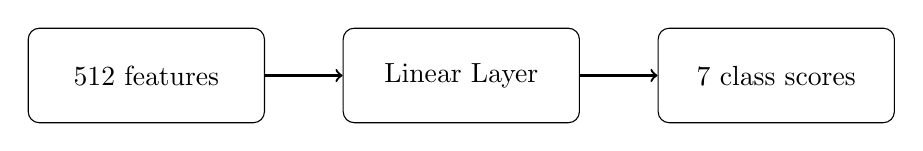
\begin{tikzpicture}[
    node distance=4cm,
    every node/.style={rectangle, rounded corners, draw, align=center, minimum width=3cm, minimum height=1.2cm},
    arrow/.style={->, thick}
]

\node (feat) {512 features};
\node (linear) [right of=feat] {Linear Layer};
\node (scores) [right of=linear] {7 class scores};

\draw[arrow] (feat) -- (linear);
\draw[arrow] (linear) -- (scores);

\end{tikzpicture}
\caption{MLP Base Head Output Layer Diagram}
\label{fig:poster_classification_head_base}
\end{figure}

Because the classification head lacks of intermediate processing, normalization, and regularization, this configuration can introduce several limitations in terms of generalization, feature refinement, and robustness for a FER task. For example: 


\begin{itemize}
    \item \textbf{Easy Overfitting:} 
    Without dropout, normalization, or nonlinear activations, the linear layer can memorize training patterns rather than learning general representations \cite{dosovitskiy_image_2021}. 

    \item \textbf{No Feature Refinement:} 
    A single linear transformation cannot abstract or transform the 512-dimensional features \cite{steiner_how_2022} \cite{tolstikhin_mlp-mixer_2021}. If some features produced by the backbone are noisy, redundant, or weakly informative, the head provides no mechanism to adjust or de-noise them.

    \item \textbf{Lack of Non-Linearity:} 
Since the head is purely linear, it cannot model complex relationships between features. This limits the expressiveness of the classifier, especially for subtle or overlapping facial expressions.

    \item \textbf{Sensitivity to Noisy Features:} 
The absence of normalization (e.g., BatchNorm) makes the classifier sensitive to variations in feature scale \cite{steiner_how_2022}. Any instability in the backbone's feature outputs directly affects classification.

    \item \textbf{No Regularization:} 
Without dropout or other regularization strategies, the head may rely too heavily on individual features, amplifying noise and making the decision boundary less stable.
\end{itemize}






\section{Proposed algorithm}

To address the base classification limitations, the current work propose an enhanced classification head that incorporates batch normalization, dropout, and a hidden non-linear projection layer. An implementation of the modified head code can be found in \ref{cod:modified_classification_head}.

 The model receives the flattened feature vector from the backbone and applies a sequence of normalization, regularization, 
and non-linear transformations before performing final classification. All the parts of the new modified head is shown in figure \ref{fig:poster_classification_head_enhanced}. 


\subsection{Design of the proposed algorithm}

%The  specific description of the design algorithm goes in this place, as well as a flow diagram with the description of how it works as seen on \textbf{Figure \ref{fig:proposedalgorithm} }
%
%\begin{figure}
%	\begin{center}
%		\includegraphics[width=1\columnwidth]{../img/image.png}
%		\caption{Example diagram.}
%		\label{fig:proposedalgorithm}
%	\end{center}
%\end{figure} 


\begin{lstlisting}[language=Python, caption={Enhanced classification head},
label={cod:modified_classification_head}]

class EnhancedHead_v1(nn.Module):
    """
    Enhanced head with BatchNorm + Dropout + Hidden Layer
    """

    def __init__(self, input_dim: int, target_dim: int, dropout_rate=0.3, hidden_ratio=0.5):
        super().__init__()
        hidden_dim = int(input_dim * hidden_ratio)

        self.features = nn.Sequential(
            nn.BatchNorm1d(input_dim),
            nn.Dropout(dropout_rate),
            nn.Linear(input_dim, hidden_dim),
            nn.ReLU(inplace=True),
            nn.BatchNorm1d(hidden_dim),
            nn.Dropout(dropout_rate / 2),
            nn.Linear(hidden_dim, target_dim)
        )

    def forward(self, x):
        x = x.view(x.size(0), -1)
        return self.features(x)

\end{lstlisting}

\begin{figure}[H]
\centering
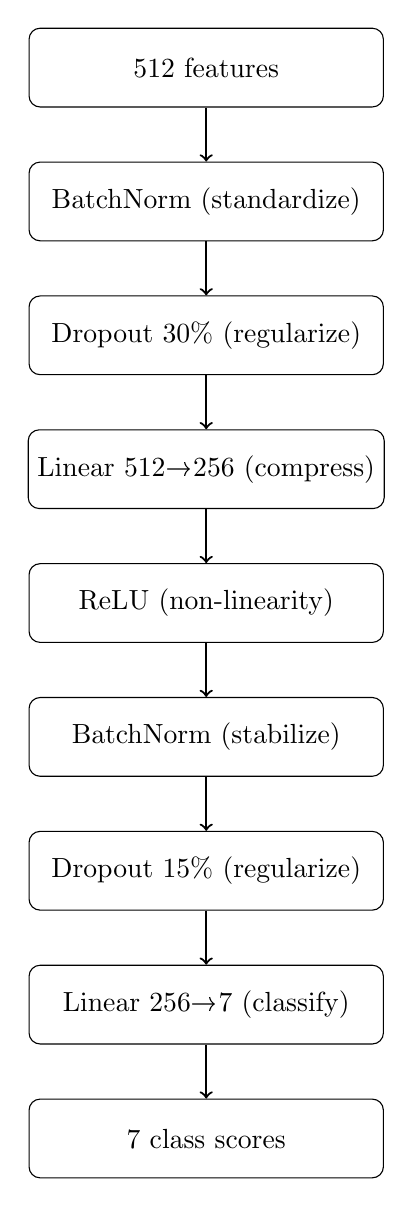
\begin{tikzpicture}[
    node distance=1.7cm,
    every node/.style={rectangle, rounded corners, draw, align=center, minimum width=4.5cm, minimum height=1cm},
    arrow/.style={->, thick}
]

\node (in) {512 features};
\node (bn1) [below of=in] {BatchNorm (standardize)};
\node (do1) [below of=bn1] {Dropout 30\% (regularize)};
\node (lin1) [below of=do1] {Linear 512→256 (compress)};
\node (relu) [below of=lin1] {ReLU (non-linearity)};
\node (bn2) [below of=relu] {BatchNorm (stabilize)};
\node (do2) [below of=bn2] {Dropout 15\% (regularize)};
\node (lin2) [below of=do2] {Linear 256→7 (classify)};
\node (out) [below of=lin2] {7 class scores};

\draw[arrow] (in) -- (bn1);
\draw[arrow] (bn1) -- (do1);
\draw[arrow] (do1) -- (lin1);
\draw[arrow] (lin1) -- (relu);
\draw[arrow] (relu) -- (bn2);
\draw[arrow] (bn2) -- (do2);
\draw[arrow] (do2) -- (lin2);
\draw[arrow] (lin2) -- (out);

\end{tikzpicture}
\caption{MLP Enhanced Head Output Layer Diagram}
\label{fig:poster_classification_head_enhanced}
\end{figure}

Some advantages of the new enhanced head include:

\begin{itemize}
    \item \textbf{Improved Generalization:} The inclusion of Dropout layers reduces overfitting, which is particularly important for FER "in-the-wild" datasets that contain relatively few samples per class.

    \item \textbf{Feature Stabilization:} Batch Normalization normalizes the intermediate feature distributions, leading to more stable gradients and faster convergence during training.

    \item \textbf{Enhanced Representational Power:} The hidden non-linear layer enables the head to refine and transform the ViT's features before classification, capturing subtle expression cues that a single linear layer cannot model.

    \item \textbf{Better Robustness to Noise:} The combination of normalization and dropout makes the head less sensitive to noisy or imperfect backbone features, which commonly occur in FER scenarios involving occlusions or variable illumination.

    \item \textbf{Modular and Lightweight:} The head introduces only a small number of additional parameters, preserving computational efficiency while significantly improving classifier capacity.

    \item \textbf{Compatible with multiple ViT's Backbone:} The enhanced head can be applied to various types of transformer architecture without modifying the underlying backbone.
    
    
\end{itemize}


\subsection{Limitations and Requirements}
A brief description of the design mechanism's limitations and requirements in accordance with the definitions in Scope and Limitations.


\subsection{Implementation}

%A brief description of the implementation and pointer to git where it can be downloaded and tested. \url{https://myalgorithm.com}.


The code of the ViT is based on the  repository\footnote{\url{https://github.com/zczcwh/POSTER}} which corresponds with the implementation of the paper \cite{zheng_poster_2022}. 

The modified version for this thesis work can be found in the following repository\footnote{\url{https://github.com/asvaaron/POSTER}}. All experiments were conducted using NVIDIA GPUs with CUDA acceleration, the table \ref{tab:hardware_used} shows more information about the available hardware. 

The training pipeline supports reproducibility through a hard-coded random seeds and modular configuration for adding the desired head changes, model sizes and hyper-parameters when training the models. The project directory structure can be found in this example \ref{lst:poster_custom_structure}.

\begin{table}[h]
\centering
\caption{Computational resources used in the experimental setup}
\label{tab:hardware_used}
\renewcommand{\arraystretch}{1.4}
\begin{tabular}{@{}l l l@{}}
\toprule
\textbf{Environment} & \textbf{Component} & \textbf{Specs} \\
\midrule
\multirow{2}{*}{Local}
 & GPU Setup & 2 × NVIDIA GeForce RTX 3060 \\
 & Machine Type & Desktop workstation \\
\midrule
\multirow{2}{*}{Cloud}
 & Platform & Google Colab Pro+ \\
 & GPU & NVIDIA GPU (variable allocation) \\
\bottomrule
\end{tabular}
\end{table}




\begin{lstlisting}[caption={Project directory structure of the POSTER implementation}, label={lst:poster_custom_structure},
%frame=none,
%basicstyle=\ttfamily\small
]

POSTER/
|-- checkpoint
|-- Confusion_matrix
|-- data
|-- data_preprocessing
|-- LICENSE
|-- log
|-- log_reader.py
|-- models
| 	|-- emotion_hyp_affect.py
|	|-- emotion_hyp.py (modified head)
|	|-- hyp_crossvit_affect.py
|	|-- hyp_crossvit.py
|	|-- ir50.py
|	|-- mobilefacenet.py
|-- README.md
|-- requirements.txt
|-- requirements_ubuntu.txt
|-- scripts_local.sh
|-- scripts.sh
|-- test_affect.py
|-- test.py
|-- torchsampler
|-- train_affect.py
|-- train.py
|-- utils.py
|-- venv
\end{lstlisting}











